\documentclass[tikz,border=5mm]{standalone}
\usepackage{tikz, pgfplots}
\usepackage[]{amsmath}
\usetikzlibrary{arrows}
\usepackage{pgfplots}
\pgfplotsset{width=8cm,compat=1.9}
\usetikzlibrary{pgfplots.dateplot}
\usepackage{pgfplotstable}
\usepackage{filecontents}
\pgfplotsset{compat=1.11}
\begin{filecontents}{date.dat}
date    value
2013-04-22  0.06
2013-05-22  0.08
2013-06-22  0.1
2013-07-22  0.2
2013-08-22  0.4
2013-09-22  1.5
2013-10-22  2.0
2013-11-22  4.1
2013-12-22  8.1
2014-01-22  15.3
2014-02-22  23.9
2014-03-22  36.5
\end{filecontents}
\begin{document}
%\pgfplotstabletypeset[string type]{date.dat}
\begin{tikzpicture}
\begin{axis}[
date coordinates in=x,
xtick=data,
xticklabel style=
{rotate=90,anchor=near xticklabel},
xticklabel=\month.\year,
title={Foo},
xlabel={Date},
y tick label style={/pgf/number format/1000 sep=},
extra y tick style={grid=major, tick label style={xshift=-1cm}},
ylabel={GH/s},
date ZERO=2009-08-18,% <- improves precision!
]
\addlegendentry{Style 1}
\addplot table[x=date,y=value] {date.dat};
\end{axis}
\end{tikzpicture}

\begin{tikzpicture}[line cap=round,line join=round,>=triangle 45,x=1.0cm,y=1.0cm]
\draw[->,color=black] (-6.72,0) -- (7.8,0);
\foreach \x in {-6,-4,-2,2,4,6}
\draw[shift={(\x,0)},color=black] (0pt,2pt) -- (0pt,-2pt) node[below] {\footnotesize $\x$};
\draw[->,color=black] (0,-3.75) -- (0,7.03);
\foreach \y in {-2,2,4,6}
\draw[shift={(0,\y)},color=black] (2pt,0pt) -- (-2pt,0pt) node[left] {\footnotesize $\y$};
\draw(3,-1) circle (2cm);
\fill [color=black] (-3,0) circle (1.5pt);
\draw [color=black] (-2.9,-0.26)-- ++(-1.5pt,-1.5pt) -- ++(3.0pt,3.0pt) ++(-3.0pt,0) -- ++(3.0pt,-3.0pt);

\begin{axis}[
    anchor=origin,  % Align the origins
    x=1cm, y=1cm,   % Set the same unit vectors
    hide axis
]
\addplot [mark=*, color=red] table {
4 5
-2 -2
-4 0
};
\addlegendentry{Style 1}
\end{axis}
\end{tikzpicture}

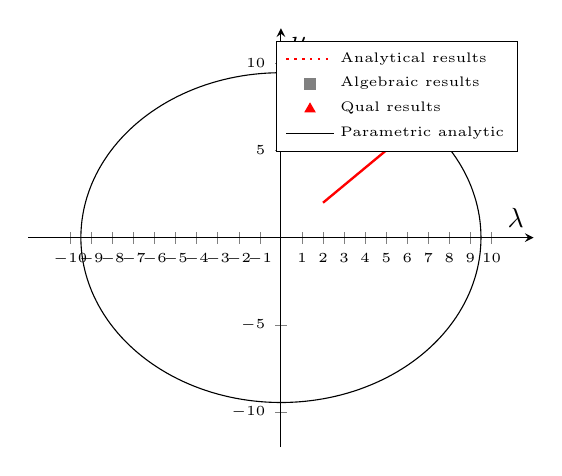
\begin{tikzpicture}
\begin{axis}[
 xlabel = $\lambda$,
 ylabel = $\nu$,
  xmin=-12,xmax=12,
  ymin=-12,ymax=12,
 %label style={font=\tiny},
  label style ={at={(ticklabel cs:1.5)}},
  xtick={-10,-9,...,10},
 tick label style={font=\tiny},
 axis lines=middle,
 legend style={font=\tiny},
 legend cell align=left,
 legend pos=north east
  ]
%%\draw[color=red,
%% line width=0.3mm] 
%% (axis cs:0.6,0.6) % moved to middle of plot to make it more visible
%%   ellipse [
%%  x radius=0.350052, y radius=0.345021];
\draw[color=red,line width=0.3mm] (02,02) -- (06,06);
\addlegendimage{line width=0.3mm,color=red,style=dotted}
\addlegendentry{Analytical results}
\addlegendimage{only marks, mark=square*,color=gray}
\addlegendentry{Algebraic results}
\addlegendimage{only marks, mark=triangle*,color=red}
\addlegendentry{Qual results}

\addplot [variable=\t,samples=200,domain=0:360] ({09.50052*cos(t)},{09.45021*sin(t)});
\addlegendentry{Parametric analytic}
\end{axis}
\end{tikzpicture}

\end{document}
%having two families of lines
%moving bounds and axes appropriately
%legend
